\section{Il "$\theta-\tau$ puzzle"}
Nel periodo iniziale delle scoperte delle particelle strane succedeva che modi di decadimento diversi venissero confusi per particelle diverse. Tuttavia, con l'aumento della precisione sulla misura delle masse si comprese di cosa si trattava. Per qualche tempo rimase un paradosso: il"$\theta-\tau$ puzzle". Due particelle (oggi si sa che è la stessa particella $K^+$):
\begin{table}[h!]
	\centering
	\renewcommand{\arraystretch}{1.5} % Aumenta lo spazio verticale tra le righe
	\begin{tabular}{|l|l|l|}
		\hline
		\textbf{Decadimento} & \textbf{$m$ (MeV)} & \textbf{$\tau$ ($10^{-8}$ s)} \\ 
		\hline
		$\theta^+ \rightarrow \pi^+ \pi^0$ & $494.0 \pm 1.0$ & $1.21 \pm 0.02$ \\ 
		\hline
		$\tau^+ \rightarrow \pi^+ \pi^+ \pi^-$ & $493.8 \pm 1.0$ & $1.19 \pm 0.05$ \\ 
		\hline
	\end{tabular}
\end{table}
Quindi stessa massa, stessa vita media ma differenti parità intrinseche. Consideriamo infatti la particella $\theta$ (di spin $S$). Lo stato inziale è un auttostato del momento angolare ma anche lo stato finale deve esserlo. Nello stato finale due particelle di spin $0$ quindi deve essere $Y_{lm}(\theta,\phi)$. Parità dello stato finale 
$$
\xi_{\pi}\xi_{\pi}(-1)^l=(-1)^l
$$
Poiché $S=l$ la particella $\theta$ può avere spin-parità: $\xi_\theta=(-1)^S$ 
$$
\left(-1 \right)^S\quad\to\quad S^\xi=0^+,1^-,2^+,3^-, \dots
$$
Consideriamo ora la particella $\tau$ che decade in $3$ pioni. Anche in questo caso un autostato del momento angolare e anche lo stato finale (3 particelle) deve essere autostato. Quindi uso la composizione di due momenti angolari: chiamo $l$ il momento angolare orbitale dei due pioni positivi e chiamo $L$ il momento angolare orbitale del pione negativo. Se lo spin della particella $\tau$ fosse $S=0$ allora
$$
|L - l| \le S \le L + l \rightarrow L = l \qquad L = l \rightarrow \xi_\tau = (-1)^3 (-1)^{l+L} = -1
$$
Quindi se $\theta$ e $\tau$ avessero spin $S=0$ avrebbero parità differente ($\xi_\theta=+1$). Per altri valori dello spin non è detto che $L=l$
$$
|L-l|\le S \le L+l
$$
Selezioniamo 2 configurazioni cinematiche che assicurino che $L$ e $l$ abbiamo valori ben definiti anche se lo spin $S$ non è nullo
\begin{itemize}
	\item $\pi^-$ ha la massima energia (mi immagino $\pi^-$ che rincula rispetto ai 2 $\pi^+$ che invece viaggiano nella stessa direzione). Quindi $\pi^+$ $\pi^+$ sono relativamente a risposo:
	$$
	l=0\to S=L \qquad \xi_\tau = (-1)^3 (-1)^L = -(-1)^S \qquad \xi_\tau \neq \xi_\theta = (-1)^S
	$$
	\item $\pi^-$ ha la minima energia ($E_{\pi^-}$=0) quindi mi immagino che il pione negativo venga prodotto a riposo e i due pioni positivi prodotti back-to-back.
	$$
	L=0\to S=l \qquad \xi_\tau = (-1)^3 (-1)^l = -(-1)^S \qquad \xi_\tau \neq \xi_\theta = (-1)^S
	$$
\end{itemize}
Sulla base di queste osservazioni Dalitz concluse che: se la particella $\tau$ decade in queste regioni cinematiche allora la sua parità è differente a quella della particella $\theta$. Cinematicamente naturalmente è possibile: occorre misurare l'elemento di matrice e il Dalitz plot.
\section{Il Dalitz Plot}
Abbiamo già studiato la cinematica del decadimento a $3$ corpi. Abbiamo visto che lo spazio delle fasi espresso in funzione delle energie di due particelle è popolato uniformemente
$$
d\Phi = \frac{1}{(2\pi)^3} \frac{1}{4} dE_1 dE_2 \qquad\frac{d\Phi}{dE_1 dE_2} = \frac{1}{(2\pi)^3} \frac{1}{4}\qquad d\Gamma = \frac{1}{2m_A} |\mathfrak{M}|^2 d\Phi_n
$$
Pertanto si misurano le energie dei prodotti di decadimento, si studia la distribuzione di questi decadimenti nel piano $E_1-E_2$, la distribuzione è quindi una misura dell'elemento di matrice. Pertanto se la parità fosse conservata l'elemento di matrice dovrebbe essere nullo nelle regioni che abbiamo individuato. Nello studio $\theta-\tau$ il Dalitz Plot è rappresentato con un triangolo equilatero. Un evento è rappresentato da un punto all'interno del triangolo. La distanza dai lati è proporzionale all'energia cinetica. Si utilizza la proprietà dei triangoli equilateri per esprimere la conservazione dell'energia $T_1+T_2+T_3=Q$. In un'approssimazione non relativistica la regione fisica è interna alla circonferenza. Inoltre dobbiamo avere simmetria fra $\pi_1$ e $\pi_2$. Il ragionamento di Dalitz era: se il decadimento della particella $\tau$ popola le regioni cinematiche $T_{\pi^-}\sim0$ e $T_{\pi^-}\sim T_{max}$ allora la sua parità è differente da quella della particella $\theta$. L'osservazione sperimentale mostra che le regioni sono popolate e pertanto o sono particelle diverse o la parità non è conservata.
\section{Esperimenti allo specchio}
Le leggi della fisica classica possiedono una proprietà di invarianza a prima vista ovvia. Consideriamo un esperimento possibile: ad esempio il modo di un oggetto sotto l'effetto del campo gravitazionale. Ciò che si ottiene osservando l'esperimento allo specchio è anch'esso un esperimento possibile e realizzabile. In tutti e due gli esperimenti la forza di gravità si calcola allo stesso modo: è diretta verso il centro della terra o, approssimativamente, verso il basso. Il moto di una massa sotto l'effetto del campo gravitazionale è invariante per riflessioni spaziali. Un altro esperimento possibile è il moto di una particella carica in presenza di un campo magnetico. La spira genera un campo magnetico (regola della mano destra). La forza di Lorentz sulla carica si calcola con la regola della mano destra. Se osserviamo lo stesso esperimento allo specchio... vediamo un esperimento realizzabile. Anche nello specchio la spira genera un campo magnetico (calcolabile con la regola della mano destra) e la forza di Lorentz si calcola con la regola della mano destra. Si sarebbe potuta usare la mano sinistra ma usare la mano destra è una convezione. Anche la riflessione di una particella in un campo magnetico invariante per riflessione spaziale. (bisogna tener conto che la fisica è invariante per rotazioni e quindi se ruoto attorno all'asse x di $\pi$ ottengo l'inversione di coordinate che è quello che voglio. Ma conviene studiare la semplice riflessione in quanto le analogie sono più comode).
\begin{figure}[h!]
	\centering
	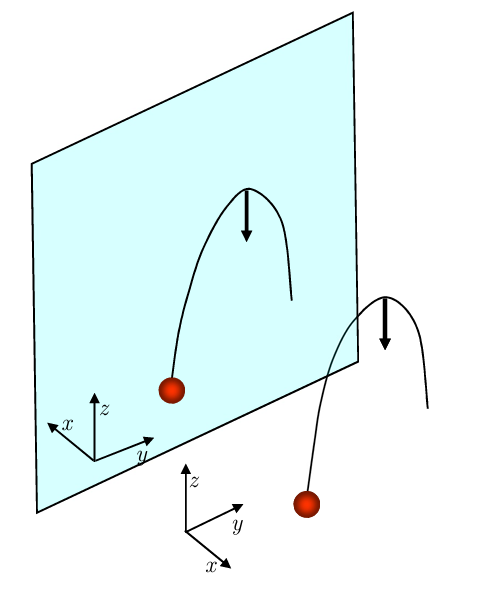
\includegraphics[width=0.4\textwidth]{Lezioni/Lezione 14/spec.png}
	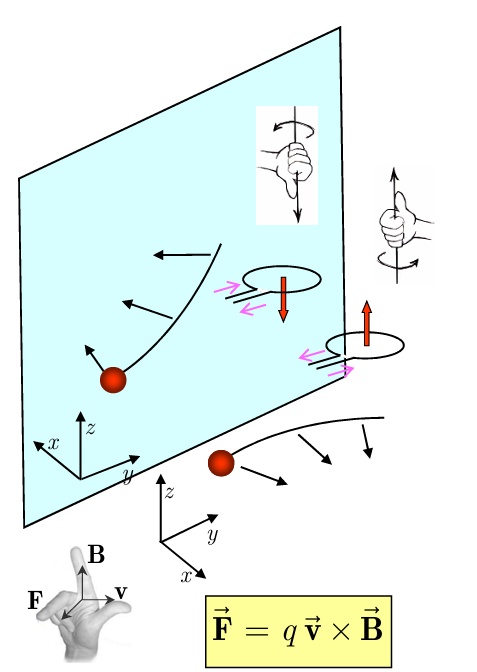
\includegraphics[width=0.4\textwidth]{Lezioni/Lezione 14/spec2.png}
	\label{fig:spec}
\end{figure}
\section{L'esperimento di Wu et al.}
Esperimento fatto nell'università di New York. La prima verifica sperimentale della violazione della parità nel decadimento $\beta$: si allineano gli spin con un campo magnetico, si scopre che il cobalto emette elettroni prevalentemente verso il basso in direzione opposta allo spin. Nell'esperimento speculare ($x\to -x$) il campo magnetico $B_z$ cambia segno; la direzione del momento magnetico $\mu$ (allineata al campo $B$) cambia segno. Se la legge fosse la stessa (e deve essere la stessa)... ci aspetteremmo pertanto che gli elettroni vadano prevalentemente verso l'alto. Invece, evidentemente, nell'esperimento nello specchio vanno verso il basso. L'esperimento visto allo specchio è impossibile. Ciò è dovuto al fatto che nell'esperimento reale si osserva una asimmetria.
\begin{figure}[h!]
	\centering
	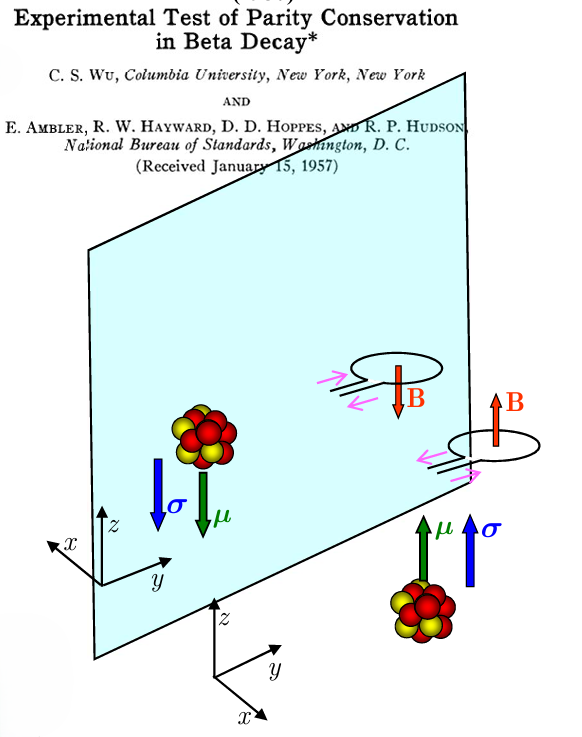
\includegraphics[width=0.4\textwidth]{Lezioni/Lezione 14/wu1.png}
	\label{fig:wu1}
\end{figure}
Per allineare gli spin occorre utilizzare temperature molto basse e un campo magnetico intenso.
\begin{figure}[h!]
	\centering
	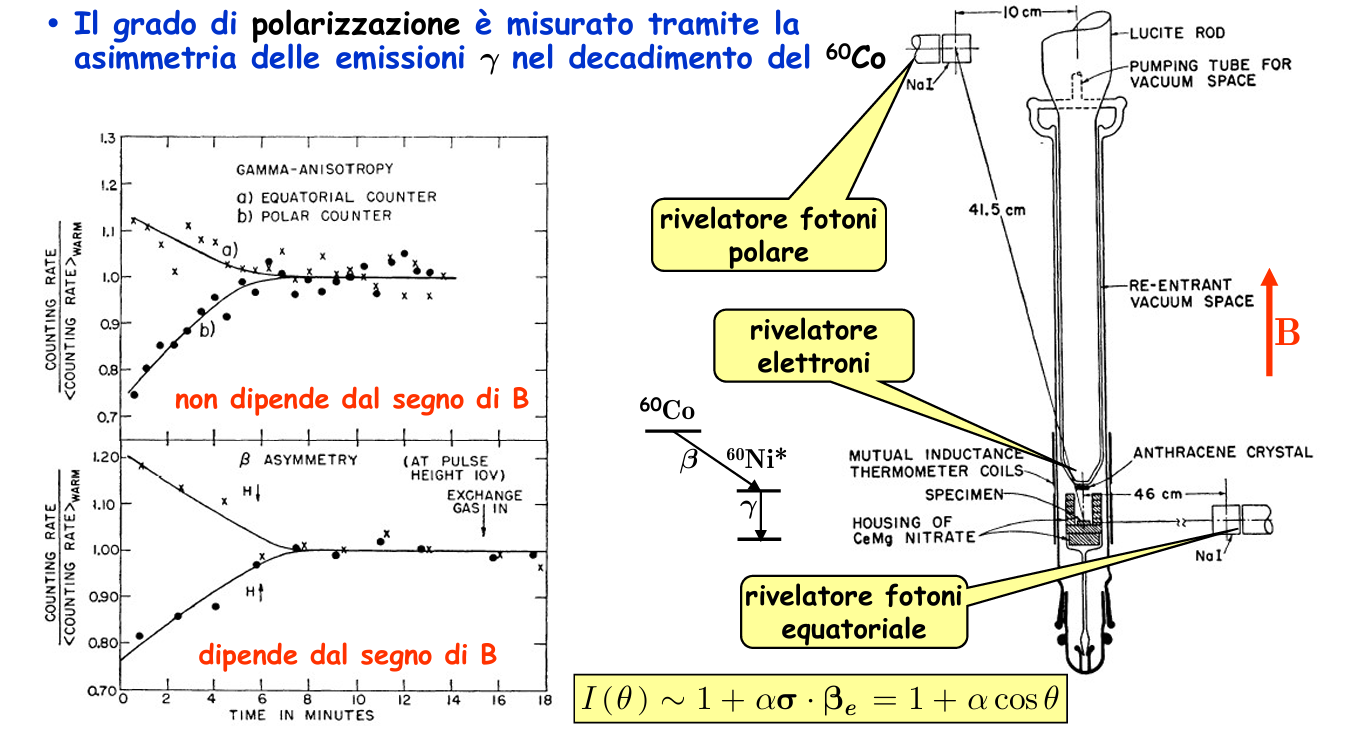
\includegraphics[width=0.9\textwidth]{Lezioni/Lezione 14/wu2.png}
	\label{fig:wu2}
\end{figure}
Il cobalto-60 non decade direttamente nel GS del Ni ma in uno stato eccitato che si diseccita elettromagneticamente con l'emissione di un fotone. Questo fotone viene utilizzato per verificare il grado di polarizzazione in quanto lo stesso Ni ha un momento angolare e quindi l'emissione non avviene in maniera isotropa. E noi andiamo a misurare l'anisotropia di questa particella misurando quanti vengono emessi in orizzontale o allineati allo spin. Quando la temperatura è bassa i due rivelatori hanno un tasso di conteggio differente quindi ho che gli spin sono allineati in quanto ho un conteggio diverso di fotoni tra rivelatore equatoriale e polare. Ma mano che alzo la temperatura conto la stessa cosa. Successivamente quindi conto quanti elettroni ho quando ho il campo magnetico verso l'alto e verso il basso. Tra l'altro la distribuzione dei fotoni non è isotropa senza dipendere dal verso del campo magnetico infatti potrei orientarlo verso l'alto o verso il basso e otterrei lo stesso grafico. Al contrario il conteggio degli elettroni cambia rispetto al segno di B!

Infatti il grafico che dimostra la violazione di parità è molto simile ma racconta una storia diversa infatti ho il conteggio di elettroni! Come asse x non c'è la temperatura perché non si sa misurare ma c'è il tempo. Infatti veniva spento il frigorifero e veniva misurato il tempo dallo stato di raffreddamento a mK a quando piano piano si scalda. Nel decadimento $\beta$ la parità è violata. 

Se avessimo fatto i calcoli su come è fatto l'elemento di matrice avremmo trovato che dentro l'elemento di matrice ($\beta_e\cdot\beta_\nu$)ci sarebbe stato un termine proporzionale al prodotto scalare velocità e direzione di volto dell'elettrone. Questa grandezza $I(\theta)$.

-Gli elettroni vanno nella direzione opposta dello spin quindi il risultato dell'esperimento allo specchio è che gli elettroni vanno verso l'alto e la violazione della parità sta proprio nel fatto che quello che vedo allo specchio sono gli elettroni che vanno verso il basso quindi il risultato che vedo allo specchio è falso-
\section{La violazione di C}
Il decadimento $\beta$ viola anche la simmetria fra particelle e antiparticelle (significa che le antiparticelle si comportano in modo diverso rispetto alle particelle). La distribuzione angolare degli elettroni (o positroni) rispetto allo spin è $I(\theta)$ che abbiamo visto prima! Il coefficiente $\alpha$ è negativo per la materia ed è positivo per l'antimateria. Questo coefficiente è diverso per il segno davanti alla massa quando vedo le equazioni $\slashed{p}\pm m$ Se nel nostro esperimento sostituiamo la materia con l'antimateria il campo magnetico cambia direzione: la corrente è di antielettroni. Il momento magnetico si allinea a $B$ e lo spin è in direzione opposta al momento magnetico in quanto ho un anti-nucleo ($Q<0$). Il coefficiente $\alpha$ diventa positivo. Nell'anti-mondo i positroni vanno verso l'alto (nel verso dello spin). 
\begin{figure}[h!]
	\centering
	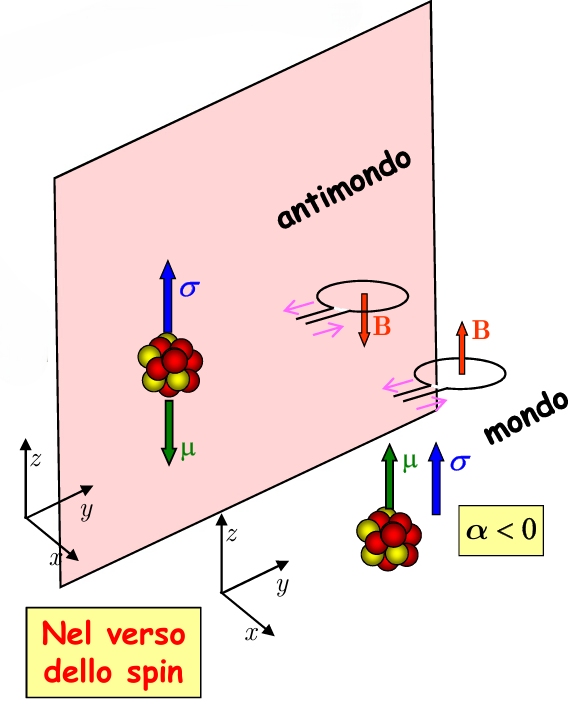
\includegraphics[width=0.7\textwidth]{Lezioni/Lezione 14/anti.png}
	\label{fig:anti}
\end{figure}
\section{Invarianza per trasformazioni CP}
Se si applicano contemporaneamente le due trasformazioni $C$ e $P$ si ottiene un esperimento possibile che produce un risultato identico all'originale. L'esperimento originale... l'esperimento allo specchio è fatto di antimateria... Il campo magnetico punta verso l'alto infatti la spira è percorsa in senso inverso ma la corrente è composta da antielettroni. Il momento magnetico punta verso l'alto e si allinea a $B$. Lo spin punta verso il basso in quanto ho un anti-nucleo e dato che si tratta di un anti-nucleo $\alpha>0$ e quindi gli elettroni vanno nella direzione dello spin verso il basso. L'interazione debole è invariante per $CP$.
\begin{figure}[h!]
	\centering
	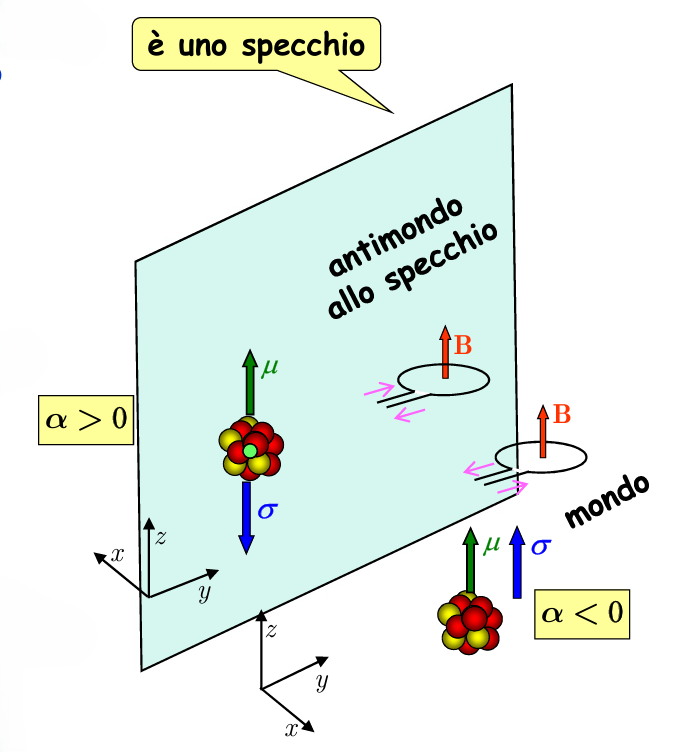
\includegraphics[width=0.7\textwidth]{Lezioni/Lezione 14/antiz.png}
	\label{fig:antiz}
\end{figure}
\section{La violazione della parità}
La scoperta che la parità è violata nei decadimenti $\beta$ impone una revisione dell'Hamiltoniana
$$
\mathcal{H}' = \sum_{i=S,V,A,T} C_i (\overline{\psi}_p \Gamma^i \psi_n) (\overline{\psi}_e \Gamma_i \psi_\nu) + h.c.
$$
In particolare la richiesta che i singoli termini debbano essere scalari non ha più una motivazione fisica. L'Hamiltoniana più generale non deve necessariamente conservare la parità: ogni termine può avere sia una parte scalare che una parte pseudo-scalare
$$
\begin{aligned}
	\mathcal{H}' &= C_S (\overline{\psi}_p \psi_n) (\overline{\psi}_e (1 + \alpha_S \gamma^5) \psi_\nu) \qquad + C_V (\overline{\psi}_p \gamma^\mu \psi_n) (\overline{\psi}_e (1 + \alpha_V \gamma^5) \gamma_\mu \psi_\nu) + \\
	&+ C_A (\overline{\psi}_p \gamma^5 \gamma^\mu \psi_n) (\overline{\psi}_e (1 + \alpha_A \gamma^5) \gamma^5 \gamma_\mu \psi_\nu) + C_T (\overline{\psi}_p \sigma^{\mu\nu} \psi_n) (\overline{\psi}_e (1 + \alpha_T \gamma^5) \sigma_{\mu\nu} \psi_\nu)
\end{aligned}
$$
Pertanto l'Hamiltoniana risulta composta da due termini
$$
\mathcal{H}' = \mathcal{H}'^{PC} + \mathcal{H}'^{PV}
$$
La parte $PV$ dell'Hamiltoniana contiene termini pseudoscalari
$$
\begin{aligned}
	\mathcal{H}'^{PV} &= \alpha_S C_S (\overline{\psi}_p \psi_n) (\overline{\psi}_e \gamma^5 \psi_\nu) \qquad + \alpha_V C_V (\overline{\psi}_p \gamma^\mu \psi_n) (\overline{\psi}_e \gamma^5 \gamma_\mu \psi_\nu) + \\
	&+ \alpha_A C_A (\overline{\psi}_p \gamma^5 \gamma^\mu \psi_n) (\overline{\psi}_e \gamma^5 \gamma^5 \gamma_\mu \psi_\nu) + \alpha_T C_T (\overline{\psi}_p \sigma^{\mu\nu} \psi_n) (\overline{\psi}_e \gamma^5 \sigma_{\mu\nu} \psi_\nu)
\end{aligned}
$$
Il termine $PC$ (Parity Conserving) è quello che abbiamo studiato fino ad ora ed è pari per trasformazioni di inversione
$$
\mathbb{P}\mathcal{H}'^{PC}\mathbb{P}^{-1} = \mathcal{H}'^{PC}
$$
Il nuovo termine $PV$ (Parity Violating) contiene prodotti di operatori che cambiano segno (odd) per trasformazioni di inversione
$$
\mathbb{P}\mathcal{H}'^{PV}\mathbb{P}^{-1} = -\mathcal{H}'^{PV}
$$
Ricordiamo che l'ampiezza di transzione è costruita con una serie perturbativa in funzione di $\mathcal{H}'$, in particolare al primo ordine
$$
\mathcal{A}_{fi} = -i \int d^4x \langle p e^- \overline{\nu} | \mathcal{H}'_I | n \rangle
$$
Una transizione è permessa se l'elemento di matrice $\mathcal{H}'$ è non nullo e una transizione è proibita se l'elemento di matrice $\mathcal{H}'$ è nullo. Consideriamo due autostati di $\mathbb{P} |a\rangle$ e $|b\rangle$ con parità intrinseca differente
$$
\mathbb{P}|a\rangle = +|a\rangle \qquad \mathbb{P}|b\rangle = -|b\rangle
$$
Si può dimostrare che
$$
\langle a | \mathcal{H}'^{PC} | b \rangle = 0 \qquad \langle a | \mathcal{H}'^{PV} | b \rangle \neq 0
$$
Cominciamo con l'elemento di matrice del termine $PC$ fra due autostati di $\mathbb{P}$ con parità diversa
$$
\begin{aligned}
	\langle a | \mathcal{H}'^{PC} | b \rangle &= \langle a | \mathbb{P}^{-1} \mathbb{P} \mathcal{H}'^{PC} \mathbb{P}^{-1} \mathbb{P} | b \rangle = (\langle a | +) \mathbb{P} \mathcal{H}'^{PC} \mathbb{P}^{-1} (- | b \rangle) \\
	&= - \langle a | \mathbb{P} \mathcal{H}'^{PC} \mathbb{P}^{-1} | b \rangle = - \langle a | (+ \mathcal{H}'^{PC}) | b \rangle = - \langle a | \mathcal{H}'^{PC} | b \rangle
\end{aligned}
$$
Quindi
$$
\langle a | \mathcal{H}'^{PC} | b \rangle = 0
$$
Calcoliamo adesso l'elemento di matrice del termine $PV$ fra due autostati di $\mathbb{P}$ con parità diversa
$$
\begin{aligned}
	\langle a | \mathcal{H}'^{PV} | b \rangle &= \langle a | \mathbb{P}^{-1} \mathbb{P} \mathcal{H}'^{PV} \mathbb{P}^{-1} \mathbb{P} | b \rangle = (\langle a | +) \mathbb{P} \mathcal{H}'^{PV} \mathbb{P}^{-1} (- | b \rangle) \\
	&= - \langle a | \mathbb{P} \mathcal{H}'^{PV} \mathbb{P}^{-1} | b \rangle = - \langle a | (- \mathcal{H}'^{PV}) | b \rangle = + \langle a | \mathcal{H}'^{PV} | b \rangle
\end{aligned}
$$
Quindi è possibile che
$$
\langle a | \mathcal{H}'^{PV} | b \rangle \neq 0
$$
Analogamente si può dimostrare che per due autostati di $\mathbb{P}$ con la stessa parità, ad esempio
$$
\mathbb{P}|a\rangle = +|a\rangle \qquad \mathbb{P}|b\rangle = +|b\rangle \qquad \Longrightarrow \qquad \langle a | \mathcal{H}'^{PC} | b \rangle \neq 0 \qquad \langle a | \mathcal{H}'^{PV} | b \rangle = 0 \qquad 
$$
\section{Conseguenze Fenomenologiche}
Le modifiche introdotte non alterano la parte nucleare e pertanto si mantiene la classificazione dei vari termini di interazione: transizioni di Fermi e transizioni di Gamov-Teller con le regole di selezione sugli spin nucleari dedotte precedentemente. Fino a quando non si studiano i processi con polarizzazione del nucleone iniziale non si hanno termini di interferenza $SA$, $ST$, $VA$, $VT$. Gli elementi di matrice si calcolano sempre utilizzando la tecnica delle tracce in particolare ricordiamo il calcolo dell'elemento di matrice di Fermi
$$
\begin{aligned}
	\overline{|\mathfrak{M}_F|^2} &= C_S^2 4m_N^2 \text{Tr}\left[(\slashed{k} + m_e)(\slashed{k}' - m_\nu)\right] \\
	&+ C_V^2 4m_N^2 \text{Tr}\left[(\slashed{k} + m_e)\gamma^0 (\slashed{k}' - m_\nu)\gamma^0\right] \\
	&+ 2 \text{Re}\left[C_S C_V 4m_N^2 \text{Tr}\left[(\slashed{k} + m_e)(\slashed{k}' - m_\nu)\gamma^0\right]\right]
\end{aligned}
$$
Assumendo $m_\nu=0$ (ipotesi non essenziale) diventa (ricordando che)
$$
\Gamma_S = 1 + \alpha_S \gamma^5 \qquad \Gamma_V = (1 + \alpha_S \gamma^5) \gamma^\mu
$$
$$
\begin{aligned}
	\overline{|\mathfrak{M}_F|^2} &= C_S^2 4m_N^2 \text{Tr}\left[(\slashed{k} + m_e)(1 + \alpha_S \gamma^5) \slashed{k}' (1 - \alpha_S \gamma^5)\right] \\
	&+ C_V^2 4m_N^2 \text{Tr}\left[(\slashed{k} + m_e)(1 + \alpha_V \gamma^5) \gamma^0 \slashed{k}' (1 + \alpha_V \gamma^5) \gamma^0\right] \\
	&+ 2 \text{Re}\left[C_S C_V 4m_N^2 \text{Tr}\left[(\slashed{k} + m_e)(1 + \alpha_S \gamma^5) \slashed{k}' (1 + \alpha_V \gamma^5) \gamma^0\right]\right]
\end{aligned}
$$
\subsection{Gli elementi di matrice}
Le tracce possono essere semplicemente sviluppate ricordando le proprietà
$$
Tr(I) = 4 \qquad Tr(\gamma^\mu \gamma^\nu) = 4g^{\mu\nu} \qquad Tr(\slashed{a}\slashed{b}) = 4a \cdot b
$$
$$
Tr(\gamma^\mu \gamma^\nu \gamma^\alpha \gamma^\beta) = 4 [g^{\mu\nu}g^{\alpha\beta} - g^{\mu\alpha}g^{\nu\beta} + g^{\mu\beta}g^{\nu\alpha}]
$$
$$
Tr(\slashed{a}\slashed{b}\slashed{c}\slashed{d}) = 4[(a \cdot b)(c \cdot d) - (a \cdot c)(b \cdot d) + (a \cdot d)(b \cdot c)]
$$
$$
Tr(\gamma^\mu) = Tr(\gamma^\mu \gamma^\nu \gamma^\delta) = Tr(\text{dispari}) = 0
$$
$$
Tr(\gamma^5) = Tr(\gamma^\mu \gamma^\nu \gamma^5) = Tr(\gamma^\mu \gamma^\nu \gamma^\delta \gamma^5) = 0
$$
$$
\begin{aligned}
	Tr(\gamma^\mu \gamma^\nu \gamma^\alpha \gamma^\beta \gamma^5) &= -4i\varepsilon^{\mu\nu\alpha\beta} \\
	Tr(\gamma_\mu \gamma_\nu \gamma_\alpha \gamma_\beta \gamma^5) &= +4i\varepsilon_{\mu\nu\alpha\beta}
\end{aligned}
$$
Per gli elementi di matrice si ottiene
$$
\overline{|\mathfrak{M}_F|^2} = 16m_N^2 E_e E_\nu \left[ C_S^2 (1 + \alpha_S^2)(1 - \boldsymbol{\beta}_e \cdot \boldsymbol{\beta}_\nu) + C_V^2 (1 + \alpha_V^2)(1 + \boldsymbol{\beta}_e \cdot \boldsymbol{\beta}_\nu) + 2C_S C_V (1 - \alpha_S \alpha_V) \frac{m_e}{E_e} \right]
$$
$$
\begin{aligned}
	\overline{|\mathfrak{M}_{GT}|^2} &= 16m_N^2 E_e E_\nu \cdot \\
	&\cdot \left[ 3C_A^2 (1 + \alpha_A^2)\left(1 - \frac{1}{3}\boldsymbol{\beta}_e \cdot \boldsymbol{\beta}_\nu \right) + 12C_T^2 (1 + \alpha_T^2)\left(1 + \frac{1}{3}\boldsymbol{\beta}_e \cdot \boldsymbol{\beta}_\nu\right) - 12C_A C_T (1 - \alpha_A \alpha_T) \frac{m_e}{E_e} \right]
\end{aligned}
$$
Consideriamo ad esempio l'elemento di matrice di Fermi. L'assenza del termine di interferenza, dedotta dallo studio della forma dello spettro, ha conseguenze meno dirette:
$$
C_SC_V\left(1-\alpha_S\alpha_V\right)=0 \quad \text{per tre condizioni} \qquad C_S=0 \quad C_V=0 \quad 1-\alpha_S\alpha_V=0
$$
Pertanto non si può più concludere che solo uno dei due accoppiamenti è attivo. Per le correlazioni angolari non ci sono sostanziali differenze. Infatti cambia solo il valore numerico delle due costanti di accoppiamento
$$
C_S^2 \to C_S^2 (1 + \alpha_S^2) \qquad C_V^2 \to C_V^2 (1 + \alpha_V^2)
$$
Occorre inventare nuovi esperimenti per determinare le nuove costanti. L'esperimento di Wu et al. fornisce le nuove informazioni necessarie. I calcoli per interpretare gli esperimenti sono però un po' più lunghi: i nuclei sono polarizzati e non si annullano i termini di interferenza Fermi/Gamow-Teller.
\section{Elettroni polarizzati}
L'osservazione della direzione privilegiata di emissione degli elettroni nell'esperimento di Wu et al. ha una implicazione molto importante sulla direzione dello spin (polarizzazione) dell'elettrone. Lo stato iniziale polarizzato $J_i=5$ di cobalto-60 mentre lo stato finale $J_f=4$ di Ni anch'esso polarizzato verso l'alto. Emette elettroni prevalentemente verso il basso quindi per conservare il momento angolare l'elettrone e il neutrino devono portare via una quantità $S=1\cdot\hbar$ di momento angolare, il neutrino e l'elettrone devono avere gli spin paralleli. Dall'esperimento di Wu gli elettroni sono emessi preferibilmente in basso (più precisamente in direzione opposta allo spin del nucleo). L'elettrone deve quindi essere polarizzato in direzione opposta alla sua direzione di moto: elettrone left-handed. Verifichiamo se l'Hamiltoniana che abbiamo scritto prevede questo fenomeno. Calcoliamo la polarizzazione degli elettroni nel decadimento $\beta$.
\subsection{Polarizzazione nel decadimento $\beta$}
La polarizzazione degli elettroni è definita
$$
\wp = \frac{N_R - N_L}{N_R + N_L}
$$
Il numero degli elettroni Right-Handed è $N_R$ e il numero degli elettroni Left-Handed è $N_L$. I numeri $N_R$ e $N_L$ sono proporzionali alle larghezze di decadimento
$$
N_{R,L} \sim \int d\Gamma_{R,L} \qquad d\Gamma_{R,L} = \frac{1}{2m_N} \overline{|\mathfrak{M}^{R,L}|^2} d\Phi
$$
Come in precedenza l'elemento di matrice contiene interazioni $S$, $V$, $A$, $T$.
$$
\mathfrak{M}^{R,L} = \mathfrak{M}_S^{R,L} + \mathfrak{M}_V^{R,L} + \mathfrak{M}_A^{R,L} + \mathfrak{M}_T^{R,L}
$$
Rivediamo i singoli termini. Osserviamo in particolare la polarizzazione degli spinori dell'elettrone
\begin{itemize}
	\item Scalare $\qquad\mathfrak{M}_S^{R,L} = C_S \langle 1 \rangle \overline{u}_e(k, s_{R,L}) (1 + \alpha_S \gamma^5) v_\nu(k') $
	\item Vettoriale $\qquad\mathfrak{M}_V^{R,L} = C_V \langle 1 \rangle \overline{u}_e(k, s_{R,L}) (1 + \alpha_V \gamma^5) \gamma^0 v_\nu(k') $
	\item Vettoriale Assiale $ \qquad\mathfrak{M}_A^{R,L} = C_A \langle \sigma_j \rangle \overline{u}_e(k, s_{R,L}) (1 + \alpha_A \gamma^5) \gamma^5 \gamma^j v_\nu(k')$
	\item Tensoriale $\qquad \mathfrak{M}_T^{R,L} = 2C_T \langle \sigma_j \rangle \overline{u}_e(k, s_{R,L}) (1 + \alpha_T \gamma^5) \Sigma^j v_\nu(k')$
\end{itemize}
Il calcolo del quadrato del modulo procede in maniera analoga a quanto fatto precedentemente sommando su tutti gli stati di polarizzazione non osservati ($n$, $p$, $\nu$). Dato che sommiamo sulla polarizzazione iniziale (del neutrone) non ci sono termini di interferenza $SA$, $ST$, $VA$, $VT$. Di nuovo abbiamo i due elementi di matrice di Fermi e di Gamow-Teller. Le somme sugli stati di polarizzazione si fanno con la tecnica delle tracce. La polarizzazione degli elettroni si introduce tramite i proiettori di spin. L'elemento di matrice di Fermi è pertanto
$$
\begin{aligned}
	\overline{|\mathfrak{M}_F^{R,L}|^2} &= C_S^2 2m_N^2 Tr \left[ (\slashed{k} + m_e) \textcolor{red}{\left(1 + \gamma^5 \slashed{s}_{R,L}\right)} (1 + \alpha_S \gamma^5) \slashed{k}' (1 - \alpha_S \gamma^5) \right] + \\
	&+ C_V^2 2m_N^2 Tr \left[ (\slashed{k} + m_e) \textcolor{red}{\left(1 + \gamma^5 \slashed{s}_{R,L}\right)} (1 + \alpha_V \gamma^5) \gamma^0 \slashed{k}' (1 + \alpha_V \gamma^5) \gamma^0 \right] + \\
	&+ 2 \text{Re} \left[ C_S C_V 2m_N^2 Tr \left[ (\slashed{k} + m_e) \textcolor{red}{\left(1 + \gamma^5 \slashed{s}_{R,L}\right)} (1 + \alpha_S \gamma^5) \slashed{k}' (1 + \alpha_V \gamma^5) \gamma^0 \right] \right]
\end{aligned}
$$
Occorre definire i vettori di polarizzazione. Il vettore $s_R$ definisce una polarizzazione parallela alla direzione di moto: polarizzazione Right-Handed. Il vettore polarizzazione $\xi$ (nel sistema di riposo) è parallelo a $k$ ($|\xi|=1$
$$
s^0 = \frac{\mathbf{k} \cdot \boldsymbol{\xi}}{m_e} \qquad s_R^0 = \frac{\mathbf{k} \cdot \boldsymbol{\xi}}{m_e} = \frac{|\mathbf{k}|}{m_e}
$$
$$
 \mathbf{s} = \boldsymbol{\xi} + \frac{(\boldsymbol{\xi} \cdot \mathbf{k})\mathbf{k}}{m_e (E_e + m_e)}
$$
$$
\begin{aligned}
	\mathbf{s}_R &= \frac{\mathbf{k}}{|\mathbf{k}|} + \frac{|\mathbf{k}|\mathbf{k}}{m_e (E_e + m_e)} = \frac{m_e (E_e + m_e) + |\mathbf{k}|^2}{m_e (E_e + m_e)|\mathbf{k}|} \mathbf{k} \\
	&= \frac{m_e E_e + E_e^2}{m_e (E_e + m_e)|\mathbf{k}|} \mathbf{k} = \frac{E_e \mathbf{k}}{m_e |\mathbf{k}|}
\end{aligned}
$$
$$
s_R = \left( \frac{|\mathbf{k}|}{m_e}, \frac{E_e}{m_e} \frac{\mathbf{k}}{|\mathbf{k}|} \right)
$$
Il vettore $s_L$ si ottiene semplicemente cambiando $\xi\to-\xi$ e quindi
$$
s_L=-s_R
$$
Ricordiamo la definizione di polarizzazione
$$
\wp = \frac{N_R - N_L}{N_R + N_L}
$$
Il numero di elettroni per le due polarizzazioni è dato da
$$
N_{R,L} \sim \int d\Gamma_{R,L} \qquad d\Gamma_{R,L} = \frac{1}{2m_N} \overline{|\mathfrak{M}^{R,L}|^2} d\Phi
$$
Pertanto la polarizzazione è data (l'integrale sullo spazio delle fasi è su tutte le variabili cinematiche escluso $E_e$ e vedremo che $\wp$ dipende dall'energia)
$$
\wp = \frac{\int \left( \overline{|\mathfrak{M}^R|^2} - \overline{|\mathfrak{M}^L|^2} \right) d\Phi}{\int \left( \overline{|\mathfrak{M}^R|^2} + \overline{|\mathfrak{M}^L|^2} \right) d\Phi}
$$
Calcoliamo il numeratore ricordando che
$$
\slashed{s}_L = -\slashed{s}_R \qquad \dots(1 + \gamma^5 \slashed{s}_R)\dots - \dots(1 + \gamma^5 \slashed{s}_L)\dots = \dots 2\gamma^5 \slashed{s}_R \dots
$$
$$
\begin{aligned}
	\overline{|\mathfrak{M}_F^R|^2} - \overline{|\mathfrak{M}_F^L|^2} &= C_S^2 2m_N^2 Tr \left[ (\slashed{k} + m_e) 2\gamma^5 \slashed{s}_R (1 + \alpha_S \gamma^5) \slashed{k}' (1 - \alpha_S \gamma^5) \right] + \\
	&+ C_V^2 2m_N^2 Tr \left[ (\slashed{k} + m_e) 2\gamma^5 \slashed{s}_R (1 + \alpha_V \gamma^5) \gamma^0 \slashed{k}' (1 + \alpha_V \gamma^5) \gamma^0 \right] + \\
	&+ 2 \text{Re} \left[ C_S C_V 2m_N^2 Tr \left[ (\slashed{k} + m_e) 2\gamma^5 \slashed{s}_R (1 + \alpha_S \gamma^5) \slashed{k}' (1 + \alpha_V \gamma^5) \gamma^0 \right] \right]
\end{aligned}
$$
Ricordando che 
$$
\wp = \frac{\int \left( \overline{|\mathfrak{M}^R|^2} - \overline{|\mathfrak{M}^L|^2} \right) d\Phi}{\int \left( \overline{|\mathfrak{M}^R|^2} + \overline{|\mathfrak{M}^L|^2} \right) d\Phi}
$$
Il numeratore (risultato del calcolo precedente) è
$$
\begin{aligned}
	\overline{|\mathfrak{M}_F^R|^2} - \overline{|\mathfrak{M}_F^L|^2} &= -8C_S^2 m_N^2 \alpha_S 4E_\nu E_e (\beta_e - \cos \theta_{e\nu}) - 8C_V^2 m_N^2 \alpha_V 4E_\nu E_e (\beta_e + \cos \theta_{e\nu}) - \\
	&+ 8(\alpha_S - \alpha_V) C_S C_V m_N^2 4m_e E_\nu \cos \theta_{e\nu}
\end{aligned}
$$
L'integrale sulle direzioni dell'elettrone e del neutrino elimina i termini dipendenti da $\cos{\theta_{e\nu}}$
$$
-8C_S^2 m_N^2 \alpha_S 4E_\nu E_e \beta_e - 8C_V^2 m_N^2 \alpha_V 4E_\nu E_e \beta_e
$$
Per quel che riguarda il denominatore notiamo che i termini $\mathfrak{M}^R$ e $\mathfrak{M}^L$ contengono rispettivamente $\frac{1}{2}(1-\gamma^5\slashed{s}_R)$ e $\frac{1}{2}(1+\gamma^5\slashed{s}_L)$. La somma di questi due termini è pertanto $1$. Il denominatore (integrato sulle direzioni) risulta uguale al risultato trovato pe la distribuzione dell'energia
$$
16m_N^2 E_e E_\nu [ C_S^2 (1 + \alpha_S^2) + C_V^2 (1 + \alpha_V^2) ]
$$
Abbiamo usato il risultato sperimentale che l'interferenza di Fierz è 0. La polarizzazione degli elettroni è pertanto
$$
\wp = \frac{-8C_S^2 m_N^2 \alpha_S 4E_\nu E_e \beta_e - 8C_V^2 m_N^2 \alpha_V 4E_\nu E_e \beta_e}{16m_N^2 E_e E_\nu \left[ C_S^2 (1 + \alpha_S^2) + C_V^2 (1 + \alpha_V^2) \right]}
$$
$$
\wp = -\beta_e \frac{2C_S^2 \alpha_S + 2C_V^2 \alpha_V}{C_S^2 (1 + \alpha_S^2) + C_V^2 (1 + \alpha_V^2)}
$$
Vedremo fra poco che gli studi sperimentali della polarizzazione degli elettroni hanno mostrato che
$$
\wp=-\beta_e
$$
Pertanto le misure sperimentali richiedono che
$$
\frac{2C_S^2 \alpha_S + 2C_V^2 \alpha_V}{C_S^2 (1 + \alpha_S^2) + C_V^2 (1 + \alpha_V^2)} = 1 \qquad 2C_S^2 \alpha_S + 2C_V^2 \alpha_V = C_S^2 (1 + \alpha_S^2) + C_V^2 (1 + \alpha_V^2)
$$
$$
C_S^2 (1 + \alpha_S^2) - 2C_S^2 \alpha_S + C_V^2 (1 + \alpha_V^2) - 2C_V^2 \alpha_V = 0
$$
$$
C_S^2 (1 - \alpha_S)^2 + C_V^2 (1 - \alpha_V)^2 = 0
$$
Ricordiamo che dalla misura della distribuzione dell'energia si conclude che il termine di interferenza di Fierz è assente. L'implicazione di questo risultato sulle costanti di accoppiamento è
$$
C_S C_V (1 - \alpha_S \alpha_V) = 0
$$
Abbiamo già notato che non possiamo trarre conlcusioni solo da questo risultato. D'altro canto, dalla misura delle correlazioni angolari
$$
a_F = \frac{C_V^2 (1 + \alpha_V^2) - C_S^2 (1 + \alpha_S^2)}{C_V^2 (1 + \alpha_V^2) + C_S^2 (1 + \alpha_S^2)} = 1
$$
Questo risultato implica
$$
C_V^2 (1 + \alpha_V^2) - C_S^2 (1 + \alpha_S^2) = C_V^2 (1 + \alpha_V^2) + C_S^2 (1 + \alpha_S^2)
$$
$$
-C_S^2 (1 + \alpha_S^2) = +C_S^2 (1 + \alpha_S^2)
$$
Da cui, come prima dell'introduzione della violazione della parità $C_S=0$ e combinando questo risultato con la misura della polarizzazione
$$
C_S^2 (1 - \alpha_S)^2 + C_V^2 (1 - \alpha_V)^2 = 0 \qquad C_V^2 (1 - \alpha_V)^2 = 0 \qquad \alpha_V=1
$$